% !TeX program = xelatex
% ============================================================
% 1981 年·全国卷（理科） · 解析版
% 由 tools/make_editions.py 生成（重跑会覆盖本文件）；
% 题目/解析内容在 questions.tex / answers*.tex，勿在本文件内写内容。
% ============================================================
\documentclass[zihao=-4, a4paper]{ctexart}
% ============================================================
% common/preamble.tex —— 拆分版试卷项目 · 公共导言区
% 引擎：XeLaTeX；文档类 ctexart 由各版本壳文件自行声明
% 由合并书 math-gaokao-2017-2026/preamble.tex 改造而来：
%   - 页眉左右改为可重定义宏 \gkheadL / \gkheadR（各版本壳设置）
%   - hyperref 不再写死 pdftitle（壳内 \hypersetup 覆盖）
%   - 删除书籍专用的 \chaptermark 重定义与 \gkpaper 装配宏
% ============================================================

% ---------- 数学 ----------
\usepackage{amsmath}
\usepackage{amssymb}
\usepackage{mathtools}

% ---------- 绘图 ----------
\usepackage{tikz}
\usetikzlibrary{shapes.geometric, arrows.meta, calc, patterns, angles, quotes, positioning}
\usepackage{pgfplots}
\pgfplotsset{compat=1.18}

% ---------- 版面 ----------
\usepackage{geometry}
\usepackage{needspace}
\geometry{a4paper, margin=2.2cm, headheight=15pt}
% 紧凑版式（如印刷版）可在壳文件中于 \begin{document} 前再次调用 \geometry 覆盖
\usepackage{enumitem}
\setlist{itemsep=2pt, topsep=4pt, parsep=0pt}

% 中文与行内公式混排的断行弹性：
% emergencystretch 允许段落末路不通时追加伸展量；
% 降低二元/关系符罚分，允许行内长公式在 = 、+ 等处断行（否则整段外溢）
\emergencystretch=2em
\binoppenalty=700
\relpenalty=500
\usepackage{booktabs}      % 三线表
\usepackage[most]{tcolorbox}

% ---------- 选择题选项对齐 ----------
% tasks 宏包：\begin{gkopts}(列数) \task ... \end{gkopts}
% 自动等宽分栏，选项天然对齐；列数已由内容片段按选项长度写定（4/2/1）
\usepackage{tasks}
\settasks{label={}, label-width=0pt, item-indent=1.2em,
          column-sep=1em, after-item-skip=2pt, before-skip=2pt, after-skip=4pt}
\NewTasksEnvironment[style=itemize]{gkopts}[\task](4)

% ---------- 页眉页脚 ----------
\newcommand{\gkheadL}{}   % 左页眉：卷名（壳文件 \renewcommand 设置）
\newcommand{\gkheadR}{}   % 右页眉：版本名（壳文件 \renewcommand 设置）
\usepackage{fancyhdr}
\pagestyle{fancy}
\fancyhf{}
\fancyhead[L]{\small\gkheadL}
\fancyhead[R]{\small\gkheadR}
\fancyfoot[C]{\small —— 第 \thepage\ 页 ——}
\renewcommand{\headrulewidth}{0.4pt}

% ---------- 超链接（须最后加载）----------
\usepackage{hyperref}
\hypersetup{colorlinks=true, linkcolor=blue!55!black,
            bookmarksnumbered=true, unicode=true}

% ============================================================
% common/macros.tex —— 自定义命令与环境（题号、解析头、提示框等）
% 与合并书 math-gaokao-2017-2026/preamble.tex 的自定义段保持一致，
% 保证内容片段（questions.tex / answers.tex）在两个项目间可互换。
% ============================================================

% ---------- 试卷标识（壳文件 \renewcommand 设置，用于 label 命名空间）----------
\newcommand{\gkpaperid}{none}

% ---------- 题号 ----------
% 试题部分的题号：加粗编号 + 自动 \label{q:<卷id>:<题号>}
\newcommand{\gkti}[1]{\par\medskip\noindent
  \textbf{#1．}\phantomsection\label{q:\gkpaperid:#1}\ignorespaces}
% 多卷/分部重启题号时，#1 是唯一内部顺序号（交叉引用身份），#2 才是原卷显示题号。
\newcommand{\gktiwithlabel}[2]{\par\medskip\noindent
  \textbf{#2．}\phantomsection\label{q:\gkpaperid:#1}\ignorespaces}

% 解析部分的题头：小标题 + 回链到试题页
% （仅在题目与解析同文档的版本中回链有效；试题版不含解析头，无悬空引用）
\newcommand{\gksolhead}[2]{%
  \Needspace{3\baselineskip}\subsubsection*{第 #1 题\if\relax\detokenize{#2}\relax\else（#2）\fi}%
  \phantomsection\label{s:\gkpaperid:#1}%
  {\small\color{gray}（题目见第~\pageref{q:\gkpaperid:#1}~页）}\par\nopagebreak}
% 与 \gktiwithlabel 成对：显示原题号，但回链仍用唯一内部顺序号。
\newcommand{\gksolheadwithlabel}[3]{%
  \Needspace{3\baselineskip}\subsubsection*{第 #2 题\if\relax\detokenize{#3}\relax\else（#3）\fi}%
  \phantomsection\label{s:\gkpaperid:#1}%
  {\small\color{gray}（题目见第~\pageref{q:\gkpaperid:#1}~页）}\par\nopagebreak}

% ---------- 填空题空位 ----------
\newcommand{\gkblank}{\underline{\hspace{2.2em}}}

% ---------- 提示框 ----------
% 卷种提示 / 解析归属声明（醒目，浅黄）
\newtcolorbox{gknotice}{colback=yellow!8, colframe=orange!60!black,
  boxrule=0.5pt, arc=1.5pt, left=6pt, right=6pt, top=4pt, bottom=4pt,
  before skip=8pt, after skip=8pt}

% 方法提示 / 注（浅蓝，用于解析后的点评与题量说明）
\newtcolorbox{gktip}{colback=blue!4, colframe=blue!35!black,
  boxrule=0.4pt, arc=1.5pt, left=6pt, right=6pt, top=4pt, bottom=4pt,
  before skip=6pt, after skip=6pt, fontupper=\small}

% ---------- 答案行 ----------
% 解析中独立成段的"答案：X"用带底色的行呈现
\newcommand{\gkanswer}[1]{\par\smallskip\noindent
  \tcbox[width=\linewidth, tcbox width=auto limited,
         colback=green!6, colframe=green!35!black, boxrule=0.4pt,
         arc=1.5pt, left=4pt, right=4pt, top=2pt, bottom=2pt,
         nobeforeafter]{\textbf{#1}}\par\smallskip}

% ---------- 结构标题 ----------
% 结构标题后通常紧跟一个带 0.5\textheight 起始预留的解析题块；0.4 只够放标题，
% 会把下一题整体推到下一页，留下孤立的「二、填空题」等页尾标题。
\newcommand{\gkpart}[1]{\Needspace{0.6\textheight}\subsection*{#1}\nopagebreak}     % 标题 + 首题
% （一）必考题 / 解析小问标题：块式加粗段，可自动换行（\paragraph 的 run-in 版式会溢出）
\newcommand{\gksubpart}[1]{\Needspace{6\baselineskip}\par\medskip\noindent\textbf{#1}\par\nopagebreak\smallskip}

% 罗马数字Ⅰ-Ⅻ（U+2160）与圈号①②③（U+2460）划入 CJK 字符类，
% 用中文字体渲染——西文字体 Latin Modern 缺这些字形，否则整段静默丢字
\xeCJKDeclareCharClass{CJK}{"2160 -> "217F, "2460 -> "24FF}

% ============================================================
% common/questions_env.tex —— 题目 / 解析的语义包装环境
%
% questions.tex 中每道题包在 \begin{question}...\end{question} 里，
% answers.tex 中每题解析包在 \begin{answer}...\end{answer} 里；
% 题头排版仍由内容行中的 \gkti / \gksolhead 完成（见 macros.tex）。
%
% 环境本身不产生任何盒子或垂直间距（只引入一个 TeX 分组），
% 排版结果与不包裹时逐点一致。它的价值在于：
%   1. 给每道题一个机器可数的结构边界（校验脚本数环境数 = 题量）；
%   2. 为将来的条件编译留钩子——某版本可重定义环境实现按题取舍。
% ============================================================

% 环境不把整题装盒：题目与解析仍可自然跨页，但开始题块前必须为题面、
% 图形/表格或解析首段留出足够空间。仅保留 2 个 baseline 会让题干、
% 选项和图形在页边界处被拆开，形成不可打印的孤立内容；题目保留
% 0.15\textheight，在避免短题制造大段空白与避免题块拆分之间取平衡。
% 解析题块保留 0.5\textheight，以容纳“题面 + 图形/选项 + 首段解析”；
% 结构标题仍用更大的保留量；末页自然收尾由视觉复审判定。
\newenvironment{question}{\Needspace{0.15\textheight}}{}
\newenvironment{answer}{\Needspace{0.5\textheight}}{}

\renewcommand{\gkpaperid}{gk-1981-regular-science}
\renewcommand{\gkheadL}{1981 年·全国卷（理科） · 数学}
\renewcommand{\gkheadR}{解析版}
\hypersetup{pdftitle={1981 年·全国卷（理科） 数学 · 解析版}}
\begin{document}
\begin{center}
  {\Large\bfseries 1981 年·全国卷（理科）}\\[4pt]
  {\large 数学 · 解析版}
\end{center}
\medskip
\pdfbookmark[1]{试题}{sec:q}
% questions.tex —— 1981 年·全国卷（理科） · 题目内容片段（无答案）
% 由 tools/generate_projects.py 依来源总账自 1981/1981_数学真题_理_试题.md 生成，勿手改（改源 MD 后重跑）


\gkpart{理科数学}

\begin{gktip}
\textbf{来源说明}：本题面依据固定原卷 PDF《1981 理》第 1 页（印刷页码 17）逐题转录。源卷为单页题面，未附答案页；配套答案与解析由本库独立推导，\textbf{非官方标准答案}。正式题为第 1—9 题；卷末「附加题」栏一题在原卷中沿用大题号印作「10．」，本库作为附加题 10 保留在第 9 题之后，不计入正式题量。第 3 题为表格题，原表第三列供填答，此处照录为空白。第 7 题附所给对数表，按原卷三列照录。
\end{gktip}

\par\medskip

\begin{question}
\gkti{1}设 $A$ 表示有理数的集合，$B$ 表示无理数的集合，即设 $A=\{\text{\text{有理数}}\}$，$B=\{\text{\text{无理数}}\}$，试写出：

（1） $A\cup B$；

（2） $A\cap B$。

\end{question}
\begin{question}
\gkti{2}在 $A$、$B$、$C$、$D$ 四位候选人中，

（1） 如果选举正、副班长各一人，共有几种选法？写出所有可能的选举结果；

（2） 如果选举班委三人，共有几种选法？写出所有可能的选举结果。

\end{question}
\begin{question}
\gkti{3}下表所列各小题中，指出 $A$ 是 $B$ 的充分条件，还是必要条件，还是充要条件，或者都不是。

\begin{center}
\begin{tabular}{lll}
\toprule
$A$ & $B$ & $A$ 是 $B$ 的什么条件 \\
\midrule
四边形 $ABCD$ 为平行四边形 & 四边形 $ABCD$ 为矩形 &  \\
$a=3$ & $\lvert a\rvert=3$ &  \\
$\theta=150^\circ$ & $\sin\theta=\dfrac12$ &  \\
点 $(a,b)$ 在圆 $x^2+y^2=R^2$ 上 & $a^2+b^2=R^2$ &  \\
\bottomrule
\end{tabular}
\end{center}

\end{question}
\begin{question}
\gkti{4}写出余弦定理（只写一个公式即可），并加以证明。

\end{question}
\begin{question}
\gkti{5}解不等式（$x$ 为未知数）：

\nopagebreak[4]
\[
\begin{vmatrix}
x-a & b & -c\\
a & x-b & c\\
-a & b & x-c
\end{vmatrix}>0.
\]

\end{question}
\begin{question}
\gkti{6}用数学归纳法证明等式：

\nopagebreak[4]
\[
\cos\frac{x}{2}\cdot\cos\frac{x}{2^2}\cdot\cos\frac{x}{2^3}\cdot\cdots\cdot\cos\frac{x}{2^n}
=\frac{\sin x}{2^n\sin\frac{x}{2^n}}.
\]

对一切自然数 $n$ 都成立。

\end{question}
\begin{question}
\gkti{7}设 1980 年底我国人口以 10 亿计算。

（1） 如果我国人口每年比上年平均递增 $2\%$，那么到 2000 年底将达到多少？

（2） 要使 2000 年底我国人口不超过 12 亿，那么每年比上年平均递增率最高是多少？

下列对数值可供选用：

\begin{center}
\begin{tabular}{lll}
\toprule
 &  &  \\
\midrule
$\lg 1.0087=0.00377$ & $\lg 1.0092=0.00396$ & $\lg 1.0096=0.00417$ \\
$\lg 1.0200=0.00860$ & $\lg 1.2000=0.07918$ & $\lg 1.3098=0.11720$ \\
$\lg 1.4568=0.16340$ & $\lg 1.4859=0.17200$ & $\lg 1.5157=0.18060$ \\
\bottomrule
\end{tabular}
\end{center}

\end{question}
\begin{question}
\gkti{8}在 $120^\circ$ 的二面角 $P-a-Q$ 的两个面 $P$ 和 $Q$ 内，分别有点 $A$ 和点 $B$，已知点 $A$ 和点 $B$ 到棱 $a$ 的距离分别为 2 和 4，且线段 $AB=10$。

（1） 求直线 $AB$ 和棱 $a$ 所成的角；

（2） 求直线 $AB$ 和平面 $Q$ 所成的角。

\Needspace{0.4\textheight}
\end{question}
\begin{question}
\gkti{9}给定双曲线 $x^2-\dfrac{y^2}{2}=1$。

（1） 过点 $A(2,1)$ 的直线 $L$ 与所给的双曲线交于两点 $P_1$ 及 $P_2$，求线段 $P_1P_2$ 的中点 $P$ 的轨迹方程；

（2） 过点 $B(1,1)$ 能否作直线 $m$，使 $m$ 与所给双曲线交于两点 $Q_1$ 及 $Q_2$，且点 $B$ 是线段 $Q_1Q_2$ 的中点？这样的直线 $m$ 如果存在，求出它的方程；如果不存在，说明理由。

\Needspace{5\baselineskip}
\textbf{附加题 10．} 已知以 $AB$ 为直径的半圆有一个内接正方形 $CDEF$，其边长为 1（如图）。设 $AC=a$，$BC=b$，作数列

\nopagebreak[4]
\[
u_1=a-b,\quad u_2=a^2-ab+b^2,\quad u_3=a^3-a^2b+ab^2-b^3,\quad\cdots,\quad
u_k=a^k-a^{k-1}b+a^{k-2}b^2-\cdots+(-1)^k b^k;
\]

求证：$u_n=u_{n-1}+u_{n-2}$（$n\geqslant 3$）。
\nopagebreak[4]
\begin{center}% 1981 年全国卷（理科）第 10 题：以 AB 为直径的半圆及其内接正方形 CDEF（按源卷布局）。
% 圆心 O 为原点、半径 sqrt(5)/2；F、C 关于 O 对称，边长为 1，E、D 在半圆上。
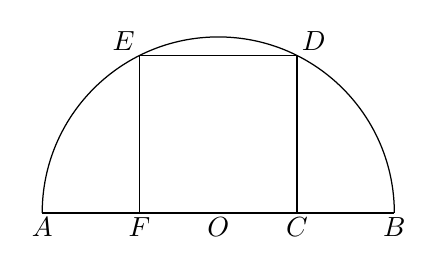
\begin{tikzpicture}[scale=2.0, line width=0.45pt,
  every node/.style={inner sep=1.5pt}]
  \pgfmathsetmacro{\R}{sqrt(5)/2}
  \coordinate (O) at (0,0);
  \coordinate (A) at (-\R,0);
  \coordinate (B) at (\R,0);
  \coordinate (F) at (-0.5,0);
  \coordinate (C) at (0.5,0);
  \coordinate (E) at (-0.5,1);
  \coordinate (D) at (0.5,1);
  % 半圆与直径 AB
  \draw (A) arc (180:0:\R);
  \draw (A) -- (B);
  % 内接正方形 CDEF
  \draw (F) -- (E) -- (D) -- (C) -- cycle;
  \node[anchor=north] at (A) {$A$};
  \node[anchor=north] at (F) {$F$};
  \node[anchor=north] at (O) {$O$};
  \node[anchor=north] at (C) {$C$};
  \node[anchor=north] at (B) {$B$};
  \node[anchor=south east] at (E) {$E$};
  \node[anchor=south west] at (D) {$D$};
\end{tikzpicture}
\end{center}
\nopagebreak[4]

\end{question}
\clearpage
\pdfbookmark[1]{参考答案与详细解析}{sec:s}
\Needspace{8\baselineskip}
\begin{center}{\Large\bfseries 参考答案与详细解析}\end{center}
\medskip
% answers.tex —— 1981 年·全国卷（理科） · 参考答案与详细解析片段
% 由 tools/generate_projects.py 依来源总账自 1981/1981_数学真题_理_试题.md + 1981/1981_数学真题_理_解析正文.md + 1981/1981_数学真题_理_答案要点.md 生成，勿手改（改源 MD 后重跑）


\begin{gknotice}
\textbf{解析归属}：本卷原卷为单页试题、未附答案页；下列各题均由本库独立推导并逐题复算，不声称代表官方标准答案。第 8 题的最终角值以反正弦形式给出并附近似度数。
\end{gknotice}

\begin{answer}
\gksolhead{1}{}

\textbf{题目}：

设 $A$ 表示有理数的集合，$B$ 表示无理数的集合，即设 $A=\{\text{\text{有理数}}\}$，$B=\{\text{\text{无理数}}\}$，试写出：

（1） $A\cup B$；

（2） $A\cap B$。

\Needspace{4\baselineskip}
\textbf{解析}

由有理数与无理数的定义，$A$ 与 $B$ 没有公共元素，且二者合起来恰好是全体实数。

\gksubpart{（1）}

\Needspace{5\baselineskip}
$A\cup B$ 由所有有理数和所有无理数组成，即全体实数的集合：

\nopagebreak[4]
\[
A\cup B=\mathbf{R}.
\]

\gksubpart{（2）}

\Needspace{5\baselineskip}
一个数不可能既是有理数又是无理数，故交集为空集：

\nopagebreak[4]
\[
A\cap B=\varnothing.
\]

\gkanswer{答案（1）：$A\cup B=\mathbf{R}$（全体实数的集合）}

\gkanswer{答案（2）：$A\cap B=\varnothing$（空集）}

\end{answer}
\begin{answer}
\gksolhead{2}{}

\textbf{题目}：

在 $A$、$B$、$C$、$D$ 四位候选人中，

（1） 如果选举正、副班长各一人，共有几种选法？写出所有可能的选举结果；

（2） 如果选举班委三人，共有几种选法？写出所有可能的选举结果。

\Needspace{4\baselineskip}
\textbf{解析}

四位候选人记为 $A$、$B$、$C$、$D$。

\gksubpart{（1）}

\Needspace{5\baselineskip}
正、副班长是两个不同职务。先定正班长，有 $4$ 种；再从余下 $3$ 人中定副班长，有 $3$ 种，故

\nopagebreak[4]
\[
4\times 3=12.
\]

\Needspace{5\baselineskip}
所有结果为有序对（正班长，副班长）：

\nopagebreak[4]
\[
(A,B),\ (A,C),\ (A,D),\ (B,A),\ (B,C),\ (B,D),\ (C,A),\ (C,B),\ (C,D),\ (D,A),\ (D,B),\ (D,C).
\]

\gksubpart{（2）}

\Needspace{5\baselineskip}
班委三人是同一职务下的组合，与顺序无关，故

\nopagebreak[4]
\[
\mathrm{C}_4^3=\frac{4\times3\times2}{3\times2\times1}=4.
\]

\Needspace{5\baselineskip}
所有结果为

\nopagebreak[4]
\[
\{A,B,C\},\quad \{A,B,D\},\quad \{A,C,D\},\quad \{B,C,D\}.
\]

\gkanswer{答案（1）：共 $4\times3=12$ 种。所有结果为（正班长，副班长）：$(A,B)$、$(A,C)$、$(A,D)$、$(B,A)$、$(B,C)$、$(B,D)$、$(C,A)$、$(C,B)$、$(C,D)$、$(D,A)$、$(D,B)$、$(D,C)$}

\gkanswer{答案（2）：共 $\mathrm{C}_4^3=4$ 种。所有结果为：$\{A,B,C\}$、$\{A,B,D\}$、$\{A,C,D\}$、$\{B,C,D\}$}

\end{answer}
\begin{answer}
\gksolhead{3}{}

\textbf{题目}：

下表所列各小题中，指出 $A$ 是 $B$ 的充分条件，还是必要条件，还是充要条件，或者都不是。

\begin{center}
\begin{tabular}{lll}
\toprule
$A$ & $B$ & $A$ 是 $B$ 的什么条件 \\
\midrule
四边形 $ABCD$ 为平行四边形 & 四边形 $ABCD$ 为矩形 &  \\
$a=3$ & $\lvert a\rvert=3$ &  \\
$\theta=150^\circ$ & $\sin\theta=\dfrac12$ &  \\
点 $(a,b)$ 在圆 $x^2+y^2=R^2$ 上 & $a^2+b^2=R^2$ &  \\
\bottomrule
\end{tabular}
\end{center}

\Needspace{4\baselineskip}
\textbf{解析}

逐行考察 $A\Rightarrow B$ 与 $B\Rightarrow A$ 是否成立。

第一行：矩形必是平行四边形，即 $B\Rightarrow A$；而平行四边形不必是矩形，$A\not\Rightarrow B$。故 $A$ 是 $B$ 的必要条件。

第二行：$a=3$ 必有 $\lvert a\rvert=3$，即 $A\Rightarrow B$；而 $\lvert a\rvert=3$ 只给出 $a=\pm3$，未必有 $a=3$，$B\not\Rightarrow A$。故 $A$ 是 $B$ 的充分条件。

第三行：$\theta=150^\circ$ 时 $\sin\theta=\sin150^\circ=\dfrac12$，即 $A\Rightarrow B$；而 $\sin\theta=\dfrac12$ 还可取 $\theta=30^\circ$ 等值，$B\not\Rightarrow A$。故 $A$ 是 $B$ 的充分条件。

第四行：点 $(a,b)$ 在圆 $x^2+y^2=R^2$ 上，按定义即 $a^2+b^2=R^2$，二者互相推出。故 $A$ 是 $B$ 的充要条件。

\gkanswer{答案：第一行（$A$：平行四边形；$B$：矩形）为必要条件；第二行（$A$：$a=3$；$B$：$\lvert a\rvert=3$）为充分条件；第三行（$A$：$\theta=150^\circ$；$B$：$\sin\theta=\frac12$）为充分条件；第四行（$A$：点 $(a,b)$ 在圆 $x^2+y^2=R^2$ 上；$B$：$a^2+b^2=R^2$）为充要条件}

\end{answer}
\begin{answer}
\gksolhead{4}{}

\textbf{题目}：

写出余弦定理（只写一个公式即可），并加以证明。

\Needspace{4\baselineskip}
\textbf{解析}

\Needspace{5\baselineskip}
余弦定理：在 $\triangle ABC$ 中，$a$、$b$、$c$ 分别为角 $A$、$B$、$C$ 的对边，则

\nopagebreak[4]
\[
a^2=b^2+c^2-2bc\cos A.
\]

\Needspace{5\baselineskip}
证明：以 $A$ 为原点、射线 $AB$ 为 $x$ 轴正方向建立直角坐标系，则

\nopagebreak[4]
\[
B(c,0),\qquad C(b\cos A,\ b\sin A).
\]

\Needspace{5\baselineskip}
由两点间距离公式，

\nopagebreak[4]
\[
a^2=BC^2=(b\cos A-c)^2+(b\sin A)^2
=b^2\cos^2A-2bc\cos A+c^2+b^2\sin^2A
=b^2+c^2-2bc\cos A.
\]

证毕。其余两式只需改换所取顶点，同理可证。

\gkanswer{答案：$\triangle ABC$ 中 $a^2=b^2+c^2-2bc\cos A$（写出等价的一式即可）}

\end{answer}
\begin{answer}
\gksolhead{5}{}

\textbf{题目}：

\Needspace{5\baselineskip}
解不等式（$x$ 为未知数）：

\nopagebreak[4]
\[
\begin{vmatrix}
x-a & b & -c\\
a & x-b & c\\
-a & b & x-c
\end{vmatrix}>0.
\]

\Needspace{4\baselineskip}
\textbf{解析}

\Needspace{5\baselineskip}
按第一行展开行列式，记 $s=b+c$：

\nopagebreak[4]
\[
D=\begin{vmatrix}
x-a & b & -c\\
a & x-b & c\\
-a & b & x-c
\end{vmatrix}
=(x-a)\bigl[(x-b)(x-c)-bc\bigr]
-b\bigl[a(x-c)-c(-a)\bigr]
+(-c)\bigl[ab-(x-b)(-a)\bigr].
\]

\Needspace{5\baselineskip}
逐项化简：

\nopagebreak[4]
\[
(x-b)(x-c)-bc=x^2-(b+c)x=x(x-s),
\]
\nopagebreak[4]
\[
a(x-c)-c(-a)=ax- ac+ac=ax,
\]
\nopagebreak[4]
\[
ab-(x-b)(-a)=ab+ax-ab=ax.
\]

\Needspace{5\baselineskip}
代入得

\nopagebreak[4]
\[
D=x(x-a)(x-s)-abx-acx
=x\bigl[(x-a)(x-s)-a(b+c)\bigr]
=x\bigl[x^2-(a+b+c)x\bigr]
=x^2\bigl(x-(a+b+c)\bigr).
\]

\Needspace{5\baselineskip}
因 $x^2\geqslant0$，故 $D>0$ 当且仅当 $x^2>0$ 且 $x-(a+b+c)>0$，即

\nopagebreak[4]
\[
x>a+b+c\ \text{且}\ x\ne0.
\]

当 $a+b+c\geqslant0$ 时，$x>a+b+c$ 已蕴含 $x>0$，此时解即 $x>a+b+c$。

复算：取 $x=0$，原行列式首行与末行互为相反数，值为 $0$，与公式 $x^2(\cdot)=0$ 一致；取 $a=b=c=0$，原行列式为 $\operatorname{diag}(x,x,x)$，值为 $x^3$，公式给出 $x^2\cdot x=x^3$，一致。

\gkanswer{答案：$x>a+b+c$ 且 $x\ne0$；当 $a+b+c\geqslant0$ 时即 $x>a+b+c$}

\end{answer}
\begin{answer}
\gksolhead{6}{}

\textbf{题目}：

\Needspace{5\baselineskip}
用数学归纳法证明等式：

\nopagebreak[4]
\[
\cos\frac{x}{2}\cdot\cos\frac{x}{2^2}\cdot\cos\frac{x}{2^3}\cdot\cdots\cdot\cos\frac{x}{2^n}
=\frac{\sin x}{2^n\sin\frac{x}{2^n}}.
\]

对一切自然数 $n$ 都成立。

\Needspace{4\baselineskip}
\textbf{解析}

\Needspace{5\baselineskip}
记

\nopagebreak[4]
\[
S_n=\cos\frac{x}{2}\cos\frac{x}{2^2}\cdots\cos\frac{x}{2^n},\qquad
T_n=\frac{\sin x}{2^n\sin\frac{x}{2^n}}.
\]

对 $n$ 用数学归纳法。

\Needspace{5\baselineskip}
$n=1$ 时，$S_1=\cos\dfrac x2$，而由二倍角公式 $\sin x=2\sin\dfrac x2\cos\dfrac x2$ 得

\nopagebreak[4]
\[
T_1=\frac{\sin x}{2\sin\frac x2}=\cos\frac x2=S_1,
\]

等式成立。

\Needspace{5\baselineskip}
假设 $n=k$ 时等式成立，即 $S_k=T_k$，则

\nopagebreak[4]
\[
S_{k+1}=S_k\cos\frac{x}{2^{k+1}}
=T_k\cos\frac{x}{2^{k+1}}
=\frac{\sin x}{2^k\sin\frac{x}{2^k}}\cdot\cos\frac{x}{2^{k+1}}.
\]

\Needspace{5\baselineskip}
由二倍角公式，取 $\theta=\dfrac{x}{2^{k+1}}$，有

\nopagebreak[4]
\[
\sin\frac{x}{2^k}=2\sin\frac{x}{2^{k+1}}\cos\frac{x}{2^{k+1}},
\qquad\text{即}\qquad
\frac{\cos\frac{x}{2^{k+1}}}{\sin\frac{x}{2^k}}=\frac{1}{2\sin\frac{x}{2^{k+1}}}.
\]

\Needspace{5\baselineskip}
代入得

\nopagebreak[4]
\[
S_{k+1}=\frac{\sin x}{2^k}\cdot\frac{1}{2\sin\frac{x}{2^{k+1}}}
=\frac{\sin x}{2^{k+1}\sin\frac{x}{2^{k+1}}}=T_{k+1},
\]

即 $n=k+1$ 时等式也成立。综上，对一切自然数 $n$ 等式成立。

\Needspace{5\baselineskip}
复算：取 $n=2$，$S_2=\cos\dfrac x2\cos\dfrac x4$，而

\nopagebreak[4]
\[
T_2=\frac{\sin x}{4\sin\frac x4}
=\frac{2\sin\frac x2\cos\frac x2}{4\sin\frac x4}
=\frac{4\sin\frac x4\cos\frac x4\cos\frac x2}{4\sin\frac x4}
=\cos\frac x4\cos\frac x2=S_2,
\]

一致。

\gkanswer{答案：见解析版}

\end{answer}
\begin{answer}
\gksolhead{7}{}

\textbf{题目}：

设 1980 年底我国人口以 10 亿计算。

（1） 如果我国人口每年比上年平均递增 $2\%$，那么到 2000 年底将达到多少？

（2） 要使 2000 年底我国人口不超过 12 亿，那么每年比上年平均递增率最高是多少？

下列对数值可供选用：

\begin{center}
\begin{tabular}{lll}
\toprule
 &  &  \\
\midrule
$\lg 1.0087=0.00377$ & $\lg 1.0092=0.00396$ & $\lg 1.0096=0.00417$ \\
$\lg 1.0200=0.00860$ & $\lg 1.2000=0.07918$ & $\lg 1.3098=0.11720$ \\
$\lg 1.4568=0.16340$ & $\lg 1.4859=0.17200$ & $\lg 1.5157=0.18060$ \\
\bottomrule
\end{tabular}
\end{center}

\Needspace{4\baselineskip}
\textbf{解析}

以 1980 年底人口 $10$ 亿为基数，2000 年底距 1980 年底为 $20$ 年。

\gksubpart{（1）}

\Needspace{5\baselineskip}
每年平均递增 $2\%$，则 20 年后人口为 $10\times(1.02)^{20}$ 亿。取对数：

\nopagebreak[4]
\[
\lg\bigl[10\times(1.02)^{20}\bigr]=1+20\lg1.02=1+20\times0.00860=1+0.17200=1.17200.
\]

\Needspace{5\baselineskip}
由所给对数表 $\lg1.4859=0.17200$，即 $10^{0.17200}=1.4859$，故

\nopagebreak[4]
\[
10\times(1.02)^{20}=10\times1.4859=14.859\approx14.86\ (\text{亿}).
\]

即到 2000 年底人口约达 $14.86$ 亿。

复算：$\ln1.02=0.0198026$，$20\ln1.02=0.396052$，$e^{0.396052}=1.485947$，与表值 $1.4859$ 相符。

\gksubpart{（2）}

\Needspace{5\baselineskip}
设每年平均递增率为 $r$，要求

\nopagebreak[4]
\[
10(1+r)^{20}\leqslant12,
\qquad (1+r)^{20}\leqslant1.2.
\]

\Needspace{5\baselineskip}
取对数：

\nopagebreak[4]
\[
20\lg(1+r)\leqslant\lg1.2=0.07918,
\qquad \lg(1+r)\leqslant0.003959.
\]

\Needspace{5\baselineskip}
所给表中 $\lg1.0092=0.00396$ 与之最接近，故

\nopagebreak[4]
\[
1+r\leqslant1.0092,\qquad r\leqslant0.0092=0.92\%.
\]

即每年比上年平均递增率最高约为 $0.92\%$。

复算：$\ln1.0092=0.009158$，$20\ln1.0092=0.18316$，$e^{0.18316}=1.20097$，略大于 $1.2$，故严格的最高递增率应略低于 $0.92\%$（约 $0.916\%$）；按所给对数表取值，答案记为约 $0.92\%$。

\gkanswer{答案（1）：约 $14.86$ 亿（$14.859$ 亿）}

\gkanswer{答案（2）：每年比上年平均递增率最高约为 $0.92\%$}

\end{answer}
\begin{answer}
\gksolhead{8}{}

\textbf{题目}：

在 $120^\circ$ 的二面角 $P-a-Q$ 的两个面 $P$ 和 $Q$ 内，分别有点 $A$ 和点 $B$，已知点 $A$ 和点 $B$ 到棱 $a$ 的距离分别为 2 和 4，且线段 $AB=10$。

（1） 求直线 $AB$ 和棱 $a$ 所成的角；

（2） 求直线 $AB$ 和平面 $Q$ 所成的角。

\Needspace{4\baselineskip}
\textbf{解析}

设 $A'$、$B'$ 分别为 $A$、$B$ 在棱 $a$ 上的射影，则 $A'A\perp a$、$B'B\perp a$，且 $A'A=2$、$B'B=4$。因 $A'A$、$B'B$ 分别在二面角的两个面内且都垂直于棱，它们所成的角即二面角的平面角，为 $120^\circ$。

\Needspace{5\baselineskip}
沿棱的方向记 $\overrightarrow{A'B'}\parallel a$，则

\nopagebreak[4]
\[
\overrightarrow{AB}=\overrightarrow{A'B'}+\overrightarrow{B'B}-\overrightarrow{A'A},
\]

\Needspace{5\baselineskip}
其中 $\overrightarrow{A'B'}$ 与另两个向量都垂直，于是

\nopagebreak[4]
\[
\lvert AB\rvert^2=A'B'^2+B'B^2+A'A^2-2\,B'B\cdot A'A\cos120^\circ
=A'B'^2+16+4-2\times4\times2\times\left(-\frac12\right)=A'B'^2+28.
\]

由 $AB=10$ 得 $A'B'^2=100-28=72$，$A'B'=6\sqrt2$。

\gksubpart{（1）}

\Needspace{5\baselineskip}
直线 $AB$ 与棱 $a$ 所成角 $\alpha$ 满足

\nopagebreak[4]
\[
\sin\alpha=\frac{\sqrt{B'B^2+A'A^2-2\,B'B\cdot A'A\cos120^\circ}}{\lvert AB\rvert}
=\frac{\sqrt{16+4+8}}{10}=\frac{\sqrt{28}}{10}=\frac{\sqrt7}{5}.
\]

\Needspace{5\baselineskip}
故

\nopagebreak[4]
\[
\alpha=\arcsin\frac{\sqrt7}{5}\approx31^\circ57'.
\]

等价地 $\cos\alpha=\dfrac{A'B'}{AB}=\dfrac{6\sqrt2}{10}=\dfrac{3\sqrt2}{5}$，与 $\sin^2\alpha+\cos^2\alpha=\dfrac7{25}+\dfrac{18}{25}=1$ 相符。

\gksubpart{（2）}

\Needspace{5\baselineskip}
在垂直于棱 $a$ 的截面内，$A'A$ 与 $Q$ 内垂直于棱的直线 $B'B$ 成 $120^\circ$ 角；因 $A'A\perp a$，它在平面 $Q$ 内的射影落在直线 $B'B$ 上，射影长为

\nopagebreak[4]
\[
A'A\cdot\lvert\cos120^\circ\rvert=2\times\frac12=1.
\]

\Needspace{5\baselineskip}
故 $A$ 到平面 $Q$ 的距离为

\nopagebreak[4]
\[
h=\sqrt{A'A^2-1^2}=\sqrt{4-1}=\sqrt3.
\]

\Needspace{5\baselineskip}
又 $B\in Q$，故直线 $AB$ 与平面 $Q$ 所成角 $\beta$ 满足

\nopagebreak[4]
\[
\sin\beta=\frac{h}{AB}=\frac{\sqrt3}{10},
\qquad
\beta=\arcsin\frac{\sqrt3}{10}\approx9^\circ58'.
\]

复算：$\sin^2\beta=\dfrac{3}{100}=0.03$，$\beta=\arcsin0.173205\approx9.975^\circ$，与上式一致。

\gkanswer{答案（1）：$\arcsin\dfrac{\sqrt7}{5}$（约 $31^\circ57'$）}

\gkanswer{答案（2）：$\arcsin\dfrac{\sqrt3}{10}$（约 $9^\circ58'$）}

\end{answer}
\begin{answer}
\gksolhead{9}{}

\textbf{题目}：

给定双曲线 $x^2-\dfrac{y^2}{2}=1$。

（1） 过点 $A(2,1)$ 的直线 $L$ 与所给的双曲线交于两点 $P_1$ 及 $P_2$，求线段 $P_1P_2$ 的中点 $P$ 的轨迹方程；

（2） 过点 $B(1,1)$ 能否作直线 $m$，使 $m$ 与所给双曲线交于两点 $Q_1$ 及 $Q_2$，且点 $B$ 是线段 $Q_1Q_2$ 的中点？这样的直线 $m$ 如果存在，求出它的方程；如果不存在，说明理由。

\Needspace{5\baselineskip}
\textbf{附加题 10．} 已知以 $AB$ 为直径的半圆有一个内接正方形 $CDEF$，其边长为 1（如图）。设 $AC=a$，$BC=b$，作数列

\nopagebreak[4]
\[
u_1=a-b,\quad u_2=a^2-ab+b^2,\quad u_3=a^3-a^2b+ab^2-b^3,\quad\cdots,\quad
u_k=a^k-a^{k-1}b+a^{k-2}b^2-\cdots+(-1)^k b^k;
\]

求证：$u_n=u_{n-1}+u_{n-2}$（$n\geqslant 3$）。
\nopagebreak[4]
\begin{center}% 1981 年全国卷（理科）第 10 题：以 AB 为直径的半圆及其内接正方形 CDEF（按源卷布局）。
% 圆心 O 为原点、半径 sqrt(5)/2；F、C 关于 O 对称，边长为 1，E、D 在半圆上。
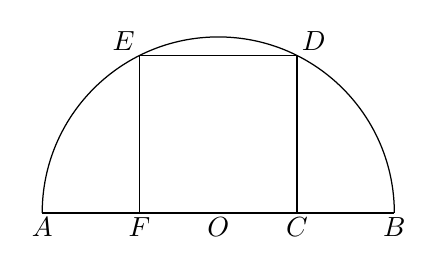
\begin{tikzpicture}[scale=2.0, line width=0.45pt,
  every node/.style={inner sep=1.5pt}]
  \pgfmathsetmacro{\R}{sqrt(5)/2}
  \coordinate (O) at (0,0);
  \coordinate (A) at (-\R,0);
  \coordinate (B) at (\R,0);
  \coordinate (F) at (-0.5,0);
  \coordinate (C) at (0.5,0);
  \coordinate (E) at (-0.5,1);
  \coordinate (D) at (0.5,1);
  % 半圆与直径 AB
  \draw (A) arc (180:0:\R);
  \draw (A) -- (B);
  % 内接正方形 CDEF
  \draw (F) -- (E) -- (D) -- (C) -- cycle;
  \node[anchor=north] at (A) {$A$};
  \node[anchor=north] at (F) {$F$};
  \node[anchor=north] at (O) {$O$};
  \node[anchor=north] at (C) {$C$};
  \node[anchor=north] at (B) {$B$};
  \node[anchor=south east] at (E) {$E$};
  \node[anchor=south west] at (D) {$D$};
\end{tikzpicture}
\end{center}
\nopagebreak[4]
\Needspace{4\baselineskip}
\textbf{解析}

\Needspace{5\baselineskip}
设弦 $P_1P_2$ 的端点为 $P_1(x_1,y_1)$、$P_2(x_2,y_2)$，中点 $P(X,Y)$，即 $x_1+x_2=2X$、$y_1+y_2=2Y$。两端点都在双曲线 $2x^2-y^2=2$ 上，两式相减：

\nopagebreak[4]
\[
2(x_1^2-x_2^2)=y_1^2-y_2^2,
\]
\nopagebreak[4]
\[
2(x_1-x_2)(x_1+x_2)=(y_1-y_2)(y_1+y_2),
\]
\nopagebreak[4]
\[
4X(x_1-x_2)=2Y(y_1-y_2).
\]

\Needspace{5\baselineskip}
当 $x_1\ne x_2$ 且 $Y\ne0$ 时，弦的斜率

\nopagebreak[4]
\[
k=\frac{y_1-y_2}{x_1-x_2}=\frac{2X}{Y}.
\]

\gksubpart{（1）}

\Needspace{5\baselineskip}
弦所在直线过 $A(2,1)$，其斜率同时又为 $\dfrac{2X}{Y}$，于是

\nopagebreak[4]
\[
\frac{2X}{Y}=\frac{Y-1}{X-2},
\qquad\text{即}\qquad
Y(Y-1)=2X(X-2),
\]

\Needspace{5\baselineskip}
整理得

\nopagebreak[4]
\[
2X^2-Y^2-4X+Y=0.
\]

\Needspace{5\baselineskip}
再验证该轨迹上的点都确能实现。取直线 $y-1=k(x-2)$，即 $y=kx+(1-2k)$，代入 $2x^2-y^2=2$：

\nopagebreak[4]
\[
(2-k^2)x^2-2k(1-2k)x-\bigl[(1-2k)^2+2\bigr]=0.
\]

\Needspace{5\baselineskip}
其判别式

\nopagebreak[4]
\[
\Delta=4k^2(1-2k)^2+4(2-k^2)\bigl[(1-2k)^2+2\bigr]
=8\bigl[(1-2k)^2+2-k^2\bigr]=8(3k^2-4k+3)>0,
\]

因为 $3k^2-4k+3$ 的判别式 $16-36<0$，恒正。故 $k\ne\pm\sqrt2$ 时直线与双曲线恒有两个不同交点。$k=\pm\sqrt2$ 时直线平行于渐近线，只交于一点，应舍去；竖直直线 $x=2$ 交双曲线于 $(2,\pm\sqrt6)$，中点为 $(2,0)$，恰是 $k\to\infty$ 的极限点。

\Needspace{5\baselineskip}
由根与系数关系亦可直接写出中点：

\nopagebreak[4]
\[
X=\frac{k(1-2k)}{2-k^2},\qquad
Y=kX+(1-2k)=\frac{2(1-2k)}{2-k^2},
\]

消去 $k$ 同样得 $2X^2-Y^2-4X+Y=0$。

\Needspace{5\baselineskip}
所以中点 $P$ 的轨迹方程为

\nopagebreak[4]
\[
2x^2-y^2-4x+y=0,
\]

\Needspace{5\baselineskip}
配方为

\nopagebreak[4]
\[
\frac{(x-1)^2}{7/8}-\frac{\left(y-\frac12\right)^2}{7/4}=1,
\]

它表示一条双曲线。

复算：取 $k=0$（直线 $y=1$），交点 $\left(\pm\sqrt{\dfrac32},1\right)$，中点 $(0,1)$，代入轨迹方程 $0-1-0+1=0$，成立；取 $k=1$（直线 $y=x-1$），交点 $(1,0)$、$(-3,-4)$，中点 $(-1,-2)$，代入 $2-4+4-2=0$，成立；取竖直弦 $x=2$，中点为 $(2,0)$，代入 $8-0-8+0=0$，成立。

\gksubpart{（2）}

\Needspace{5\baselineskip}
反设存在这样的直线 $m$。设 $m$ 与双曲线交于 $Q_1(x_1,y_1)$、$Q_2(x_2,y_2)$，$B(1,1)$ 为中点，则 $x_1+x_2=2$、$y_1+y_2=2$，由前述斜率公式，$m$ 的斜率必为

\nopagebreak[4]
\[
k=\frac{2X}{Y}=\frac{2\times1}{1}=2.
\]

\Needspace{5\baselineskip}
于是 $m$ 只能是过 $B$ 且斜率为 $2$ 的直线：

\nopagebreak[4]
\[
y-1=2(x-1),\qquad y=2x-1.
\]

\Needspace{5\baselineskip}
把它代入 $2x^2-y^2=2$：

\nopagebreak[4]
\[
2x^2-(2x-1)^2=2
\ \Longrightarrow\
-2x^2+4x-3=0
\ \Longrightarrow\
2x^2-4x+3=0.
\]

\Needspace{5\baselineskip}
其判别式

\nopagebreak[4]
\[
\Delta=(-4)^2-4\times2\times3=16-24=-8<0,
\]

方程无实根，即直线 $y=2x-1$ 与双曲线没有公共点，与「交于两点」矛盾。故这样的直线 $m$ 不存在。

复算：$-2x^2+4x-3=0$ 两边乘 $-1$ 得 $2x^2-4x+3=0$，$\Delta=16-24=-8$，确无实交点。

\textbf{附加题 10}

\Needspace{4\baselineskip}
\textbf{解析}

先由图形求出 $a$、$b$ 的两个关系。设圆心为 $O$（$AB$ 的中点），半径为 $R$，则 $AB=a+b=2R$。

\Needspace{5\baselineskip}
正方形上边 $ED$ 是圆的弦，且 $ED\parallel AB$，故 $O$ 在 $AB$ 上的射影是 $ED$ 的中点，也就是 $FC$ 的中点；于是 $F$、$C$ 关于 $O$ 对称，

\nopagebreak[4]
\[
OF=OC=\frac12 FC=\frac12.
\]

\Needspace{5\baselineskip}
又

\nopagebreak[4]
\[
OC=AC-AO=a-\frac{a+b}{2}=\frac{a-b}{2},
\]

\Needspace{5\baselineskip}
故

\nopagebreak[4]
\[
\frac{a-b}{2}=\frac12,\qquad a-b=1.
\]

\Needspace{5\baselineskip}
再由点 $D$ 在圆上：$OD=R=\dfrac{a+b}{2}$，而 $O$ 到 $D$ 的水平距离为 $\dfrac12$、竖直距离为 $1$（正方形边长），故

\nopagebreak[4]
\[
OD^2=\left(\frac12\right)^2+1^2=\frac54,
\qquad
\frac{a+b}{2}=\frac{\sqrt5}{2},
\qquad
a+b=\sqrt5.
\]

\Needspace{5\baselineskip}
于是

\nopagebreak[4]
\[
ab=\frac{(a+b)^2-(a-b)^2}{4}=\frac{5-1}{4}=1.
\]

\Needspace{5\baselineskip}
下面证递推式。由定义把 $u_n$ 的首项分出，其余各项提出公因子 $-b$：

\nopagebreak[4]
\[
u_n=a^n-a^{n-1}b+a^{n-2}b^2-\cdots+(-1)^n b^n
=a^n-b\bigl(a^{n-1}-a^{n-2}b+\cdots+(-1)^{n-1}b^{n-1}\bigr)
=a^n-b\,u_{n-1}.
\]

\Needspace{5\baselineskip}
对 $u_{n-1}$ 用同一恒等式，得

\nopagebreak[4]
\[
u_{n-1}=a^{n-1}-b\,u_{n-2}.
\]

\Needspace{5\baselineskip}
把后式两边乘以 $a$：

\nopagebreak[4]
\[
a\,u_{n-1}=a^n-ab\,u_{n-2}=a^n-u_{n-2}
\qquad(\text{因 }ab=1),
\]

\Needspace{5\baselineskip}
即

\nopagebreak[4]
\[
a^n=a\,u_{n-1}+u_{n-2}.
\]

\Needspace{5\baselineskip}
代回前式：

\nopagebreak[4]
\[
u_n=a\,u_{n-1}+u_{n-2}-b\,u_{n-1}
=(a-b)u_{n-1}+u_{n-2}
=u_{n-1}+u_{n-2}
\qquad(\text{因 }a-b=1).
\]

原式得证。

\Needspace{5\baselineskip}
复算：由 $a-b=1$ 与 $ab=1$ 得 $a^2-a-1=0$、$b^2+b-1=0$。取 $a=\dfrac{\sqrt5+1}{2}$、$b=\dfrac{\sqrt5-1}{2}$，则

\nopagebreak[4]
\[
u_1=a-b=1,\qquad
u_2=a^2-ab+b^2=(a+b)^2-3ab=5-3=2,
\]
\nopagebreak[4]
\[
u_3=a^3-a^2b+ab^2-b^3=(a-b)(a^2+b^2)=1\times\bigl((a+b)^2-2ab\bigr)=5-2=3.
\]

而 $u_2+u_1=2+1=3=u_3$，递推式在 $n=3$ 处成立；继续 $u_4=u_3+u_2=5$，与由 $u_k=a^k-b\,u_{k-1}$ 逐步算得的结果一致。

\gkanswer{答案（1）：$2x^2-y^2-4x+y=0$（即 $\dfrac{(x-1)^2}{7/8}-\dfrac{\left(y-\frac12\right)^2}{7/4}=1$，为一条双曲线）}

\gkanswer{答案（2）：不存在}

\end{answer}
\end{document}
